\clearpage
\title{Adding Two Numbers}
\author{}
\date{}
\maketitle

\section*{Tools Used}
\begin{itemize}
    \item emu8086 - 8086 Microprocessor Emulator
    \item MacTeX -\LaTeX  compiler.
    \item VS Code with \LaTeX workshop extension as a text editor.
\end{itemize}

\section*{Process}

\subsection*{Code:}
\begin{minted}[breaklines, linenos]{gas}
DATA    SEGMENT
    CR EQU 0DH
    LF EQU 0AH

    MSG1 DB 'ENTER FIRST NUMBER: $'
    NUM1 DB ?
    MSG2 DB CR,LF,'ENTER SECOND NUMBER: $'
    NUM2 DB ?
    MSG3 DB CR, LF, 'SUM = '
    NUM3 DW ?,'$'
DATA    ENDS

CODE    SEGMENT
    ASSUME CS:CODE, DS:DATA
    
START: 
    MOV AX, DATA
    MOV DS, AX
           
    LEA DX, MSG1
    MOV AH, 9
    INT 21h
    
    MOV AH, 1
    INT 21h
    SUB AL, '0'  
    MOV NUM1, AL
    
    LEA DX, MSG2
    MOV AH, 9
    INT 21h
    
    MOV AH, 1
    INT 21h
    SUB AL, '0' 
    MOV NUM2, AL
    
    MOV BH,0
    MOV BL, NUM1
    MOV AH, 0  
    MOV AL, NUM2
    ADD AX,BX
    MOV NUM3, AX
    
    ADD NUM3, '0'
    
    LEA DX, MSG3
    MOV AH, 9
    INT 21h
    
    MOV AH, 4CH
    INT 21h
     
CODE    ENDS

END START
\end{minted}

\subsection*{Output}
\begin{center}
    \centering
    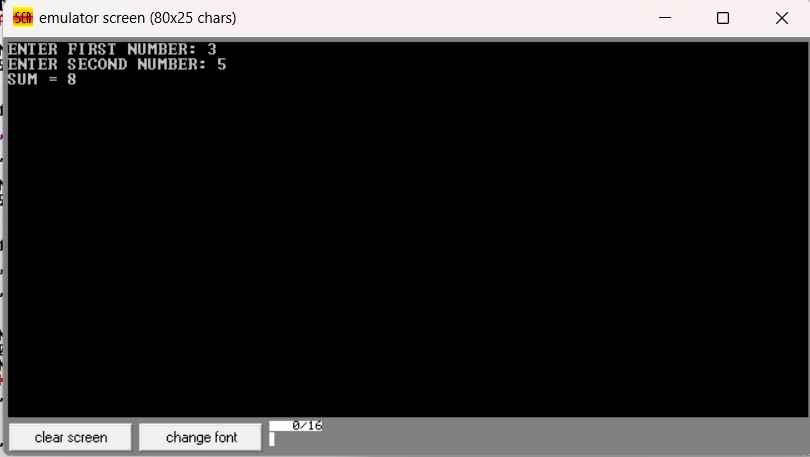
\includegraphics[width = .8\textwidth]{MALI3.jpg}
    \captionof{figure}{Uppercase to Lowercase}
\end{center}
